En esta primera práctica nos familiarizaremos con las interfaces gráficas del
QGIS y de R-studio analizando la imagen Landsat 8 de noviembre de
2016, desde el punto de vista espectral. Son nuestros objetivos:

\begin{itemize}
    \item Abrir una imagen en QGIS.
    \item Crear archivos vectoriales y digitalizar coberturas en QGIS.
    \item Abrir un archivo raster y vectorial en R.
    \item Realizar un análisis estad\'istico de la imagen y de las
        distintas coberturas digitalizadas en R.
\end{itemize}
\section{Exploración de im\'agenes con el QGIS}

Comenzamos abriendo la imagen \file{LC82240782016304LGN00.vrt} que se encuentra
en la carpeta \file{raster\_data,LC82240782016304}, la cual  corresponde al
departamento de Iguaz\'u en la provincia de Misiones. Fue obtenida por
el satelite Landsat 8 durante el mes de noviembre de 2016.

En el menú \menu{Capa, Añadir capa, Añadir capa ráster}. Navegamos
hasta la carpeta \file{raster\_data/LC8224078201630} y abrimos la imagen
\file{LC82240782016304LGN00.vrt}. La encontraremos
en el \menu{Panel de capas} de QGIS. Podemos usar las herramientas para
movernos en la imagen (Figura \ref{fig:move}).

\begin{figure}[h!]
\begin{center}
    
\includegraphics[scale=0.5]{move.png}
\end{center}
\caption{Herramientas para moverse dentro de la imagen. De izquierda a derecha:
    1. Desplazar mapa, 2. Desplazar mapa a la selecci\'on, 3. Acercar zoom, 4.
    Alejar zoom, 5. zoom a la resolucion nativa, 6. zoom general, 7. zoom a la
    selecci\'on, 8. zoom a la capa, 9. zoom anterior, 10. zoom siguiente, 11.
    Actualizar.}
\label{fig:move}
\end{figure}

Para realizar cambios en la visualizaci\'on y explorar las propiedades de una
capa, hacemos click derecho sobre ella y luego seleccionamos la opci\'on
\menu{Propiedades}. All\'i podemos ir a la pestaña
\menu{General} para ver datos como el nombre de la capa\footnote{Es un buen
momento para ponerle uno mas sencillo}, la cantidad de filas y columnas del
archivo, el valor digital no v\'alido, el sistema de coordenadas
entre otros (Figura \ref{fig:general}).

\begin{figure}[h!]
\begin{center}
    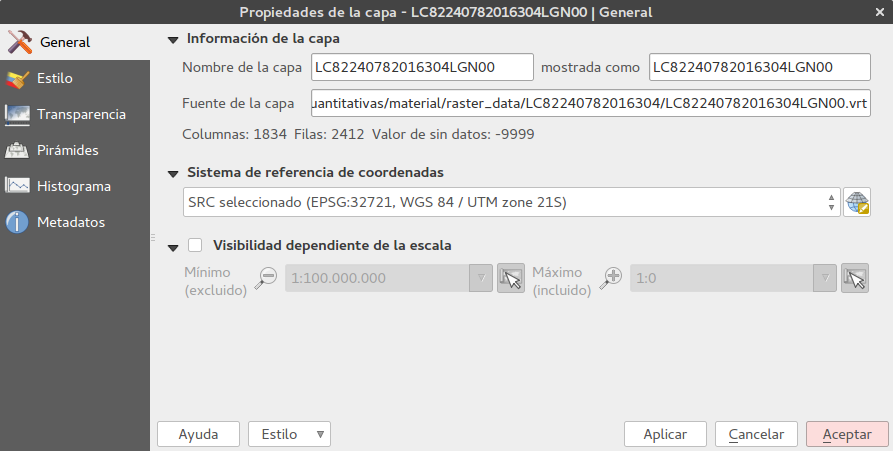
\includegraphics[scale=0.4]{general.png}
\end{center}
\caption{Pestaña general de propiedades de una capa. Podemos ver
    los datos m\'as importantes como la cantidad de filas y
    columnas, el nombre y el sistema de referencia.}
\label{fig:general}
\end{figure}

En la pestaña \menu{Estilo} podemos cambiar la visualizaci\'on de
la capa. All\'i elegimos de que color mostrar cada una de las
bandas. Para cambiar el realce hacemos
click en el boton \menu{Cargar} para seleccionar los valores m\'aximos y m\'inimos
(Figura \ref{fig:estilo}).

\begin{figure}[h!]
\begin{center}
    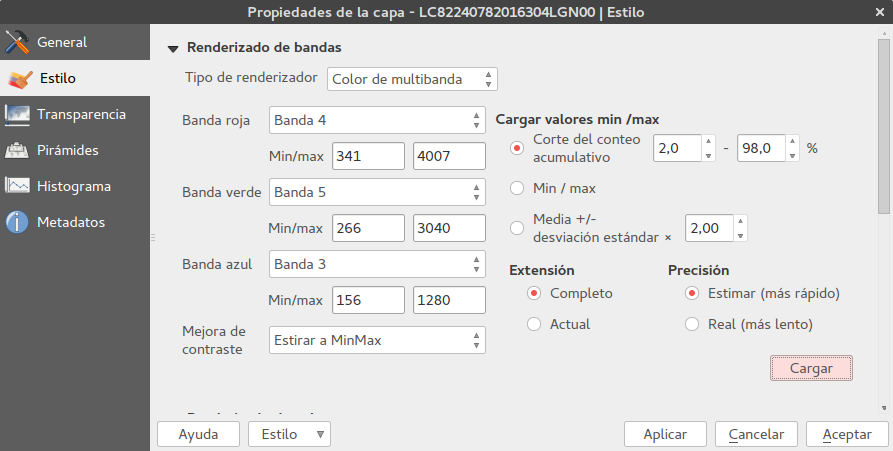
\includegraphics[scale=0.4]{estilo.png}
\end{center}
\caption{Estilos de visualizaci\'on de una capa raster.}
\label{fig:estilo}
\end{figure}

La herramienta \menu{Identificar un objeto espacial} nos permite extraer valores
de la imagen. Al habilitarla veremos datos como el valor
de reflectancia del p\'ixel seleccionado que pueden mostrarse como
\'Arbol, Tabla o Grafo seg\'un uno desee (Figura \ref{fig:grafo}).

\begin{figure}[h!]
\begin{center}
    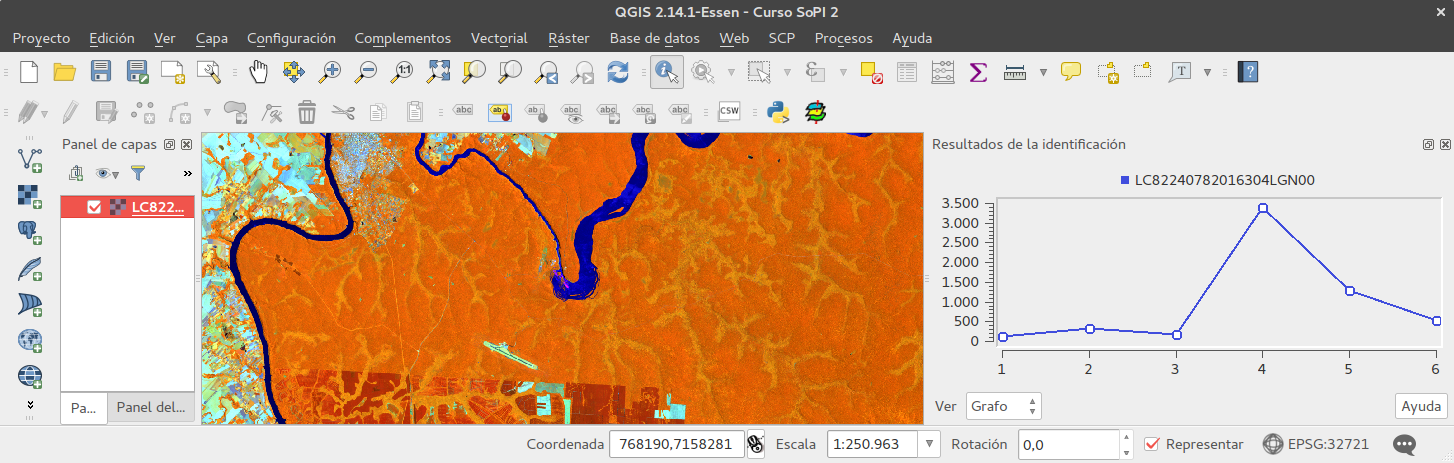
\includegraphics[scale=0.2]{grafo.png}
\end{center}
\caption{Identificaci\'on de un p\'ixel correspondiente a la selva paranaense
    mostrada como grafo. }
\label{fig:grafo}
\end{figure}

\begin{act}
    Cambie la combinación de bandas de la imagen Landsat 8 a color real y expl\'orela.
    Identifique zonas de coberturas uniformes. Pruebe cambiar de
    combinaci\'on de bandas y decida si las zonas siguen siendo uniformes
    despu\'es de cada cambio.
\end{act}

\begin{act}
    Encuentre el sistema de coordenadas en el cual se obtenga la imagen.
    ¿Cu\'antas filas y columnas tiene?
\end{act}

\begin{act}
   Utilizando la herramienta identificar objetos espaciales encuentre los
   valores de reflectancia de distintas coberturas. Grafique estos  valores en
   funci\'on de la longitud de onda y en el espacio espectral.
\end{act}

\section{Creaci\'on de capas vectoriales}

La capas vectoriales nos ser\'a de utilidad en este curso, para extrar datos
cuantitativos de las capas raster.

Con la herramienta \menu{nueva capa de archivo shape} es posible crear una nueva
capa vectorial. Para esto hacemos click en el bot\'on que se
encuentra en el panel lateral. Podemos agregar los campos que sean necesarios
para nuestra capa vectorial. En este caso, ser\'an los campos: MC\_ID, como
entero de longitud 1 y Comment, como texto de 80 caracteres. Elegimos el sistema
de coordenadas correspondiente a la imagen anterior, guardamos en la carpeta
\file{vector\_data/}, con el nombre \file{firmas.shp} (Figura \ref{fig:newshape}).

\begin{figure}[h!]
\begin{center}
    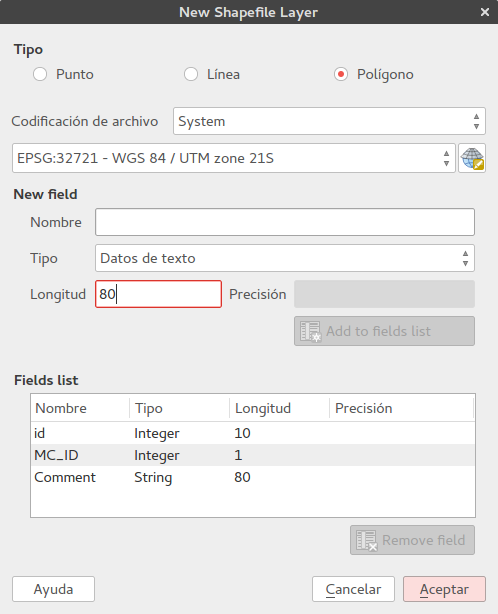
\includegraphics[scale=0.4]{new_shape.png}
\end{center}
\caption{Creaci\'on de una nueva capa vectorial.}
\label{fig:newshape}
\end{figure}


Una vez creada, utilizamos la barra de herramientas de QGIS, (Figura \ref{fig:shapetool}),
para agregarle geometr\'ias. Para esto hacemos click en el bot\'on
de agregar geometr\'ia y digitalizamos una zona uniforme dentro de la imagen.
\begin{figure}[h!]
\begin{center}
    
\includegraphics[scale=0.5]{shapetool.png}
\end{center}
\caption{Herramientas de edición vectorial. De izquierda a derecha: 1. Conmutar
    edici\'on, 2. Guardar cambios a la capa, 3. Añadir objeto espacial, 4. Añadir
    cadena circular, 5. Mover objeto espacial, 6. Herramienta de nodos, 7.
    Borrar lo seleccionado, 8. Cortar objetos espaciales, 9. Copiar objetos
    espaciales, 10. Pegar objetos espaciales.}
\label{fig:shapetool}
\end{figure}

Al terminar, QGIS pedir\'a un n\'umero de ID para la capa que debe ser
correlativo. Además podremos ingresar en este momento los valores del resto de
los campos de nuestro objeto espacial (Figura \ref{fig:newpoli}).

\begin{figure}[h!]
\begin{center}
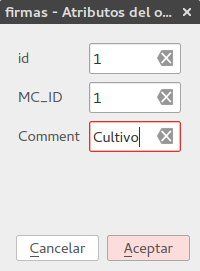
\includegraphics[scale=0.4]{new_poli.png}
\end{center}
\caption{Valores de los campos del nuevo poligono creado.}
\label{fig:newpoli}
\end{figure}

Es importante recordar que debemos estar en el modo de edici\'on para poder hacerlo.
Al terminar debemos desactivar esa opci\'on.

\begin{act}
   Digitalice coberturas uniformes dentro de la imagen. Recuerde obtener al
   menos un pol\'igono por cada categor\'ia de uso y cobertura presente.
\end{act}

En caso de necesitar cambiar la visualizaci\'on de la capa vectorial, podemos entrar
a sus propiedades\footnote{Pueded utilizar el estilo precargado
ubicado en la carpeta \file{aux\_data}}. Podemos acceder a la tabla de
datos de la capa vectorial haciendo click derecho sobre ella y eligiendo la
opci\'on \menu{Abrir tabla de atributos}.

\section{Exploraci\'on raster en R}

Veamos como abrir y trabajar con las im\'agenes satelitales en R. La forma de
realizar operaciones es escribir comandos en la consola de R-studio y
ejecutarlos presionando enter. Para trabajar con im\'agenes satelitales debemos utilizar
algunas librerias adicionales. Para cargarlas usamos el comando
\texttt{library(raster)}. De esta forma agregamos funciones que nos facilitaran
el trabajo raster.

Adem\'as, deberemos situar nuestra carpeta de trabajo donde se encuentran las
carpetas que descargamos. Para esto nos movemos en el explorador de archivos
hasta ella y hacemos click en usar la carpeta como carpeta de trabajo (Figura \ref{fig:setwd}).

\begin{figure}[h!]
\begin{center}
    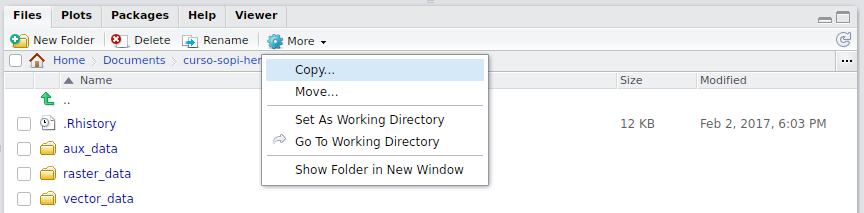
\includegraphics[scale=0.4]{setwd.png}
\end{center}
\caption{Configuraci\'on del directorio de trabajo desde la interfaz gr\'afica.}
\label{fig:setwd}
\end{figure}

Tambi\'en podemos utilizar el comando \texttt{setwd(.)} para configurar el
directorio de trabajo. En este caso hay que especificar la ruta completa hasta
\'el.

Una vez en la carpeta, existen varias maneras de abrir una imagen. Con el comando
\texttt{raster}, abrimos una \'unica banda; \texttt{brick}, abrimos un archivo multibanda,
;y \texttt{stack}, abrimos distintas bandas por separado. Veamos algunos ejemplo:

\begin{exa}
    Abrimos la imagen completa del archivo de Landsat 8 y consultamos sus
    propiedades.
    \begin{lstlisting}
    ref.2016 <- brick("raster_data/LC82240782016304/LC82240782016304LGN00.vrt")
    ref.2016
    \end{lstlisting}
    obtenemos de resultado el siguiente texto
    \begin{Verbatim}[fontsize=\small]
    class       : RasterBrick
    dimensions  : 2412, 1834, 4423608, 6  (nrow, ncol, ncell, nlayers)
    resolution  : 30.00402, 30.00265  (x, y)
    extent      : 731118.6, 786146, 7101531, 7173897  (xmin, xmax, ymin, ymax)
    coord. ref. : +proj=utm +zone=21 +south +datum=WGS84 +units=m +no_defs
                  +ellps=WGS84 +towgs84=0,0,0
    data source : ./material/raster_data/LC82240782016304/LC82240782016304LGN00.vrt
    names       : LC82240782016304LGN00.1, LC82240782016304LGN00.2, ...
    min values  :                     -33,                     192, ...
    max values  :                    2774,                    3265, ...
    \end{Verbatim}
    En \'el, podemos ver la clase a la que corresponde el archivo, en este
    caso un \emph{RasterBrick}, las dimensiones, el tamaño de p\'ixel, extensi\'on
    de la capa, proyecci\'on, cual es la ruta al archivo, las bandas y
    sus valores m\'aximos y m\'inimos.

    Cambiemos el nombre a las bandas y la convertimos a reflectancia entre 0 y 1.

    \begin{lstlisting}
    names(ref.2016) <- c("blue","green","red","nir","swir1","swir2")
    ref.2016 <- ref.2016/1e4
    rasterOptions(addheader = "ENVI")
    writeRaster(ref.2016,"raster\_data/processed/ref2016")
    \end{lstlisting}

    Analicemos el c\'odigo l\'inea por l\'inea.
    \begin{itemize}
    \item La primera abre la imagen como  un raster de m\'ultiples bandas.
    \item La segunda, cambia los nombres de cada banda a los que figuran en la
          lista entre par\'entesis. Es importante resaltar que el n\'umero de nombres
          debe ser el mismo que el de bandas.
    \item En tercer lugar, convertimos el archivo de n\'umeros enteros entre 0 y
          10000 a valores entre 0 y 1.
    \item La cuarta linea es necesaria correrla una sola vez por sesi\'on. La misma
          agrega el header de ENVI a nuestro output para poder abrir el archivo
          desde QGIS
      \item La quinta l\'inea guarda el archivo raster con el nombre \file{ref2016}
          . En este caso estamos usando el formato nativo de R.
    \end{itemize}
    Podemos graficar una combinacion de bandas con el comando
    \texttt{plotRGB(ref.2016,r=4,g=5,b=3, stretch='lin')}(Figura \ref{fig:plot453})

    \begin{figure}[h!]
    \begin{center}
        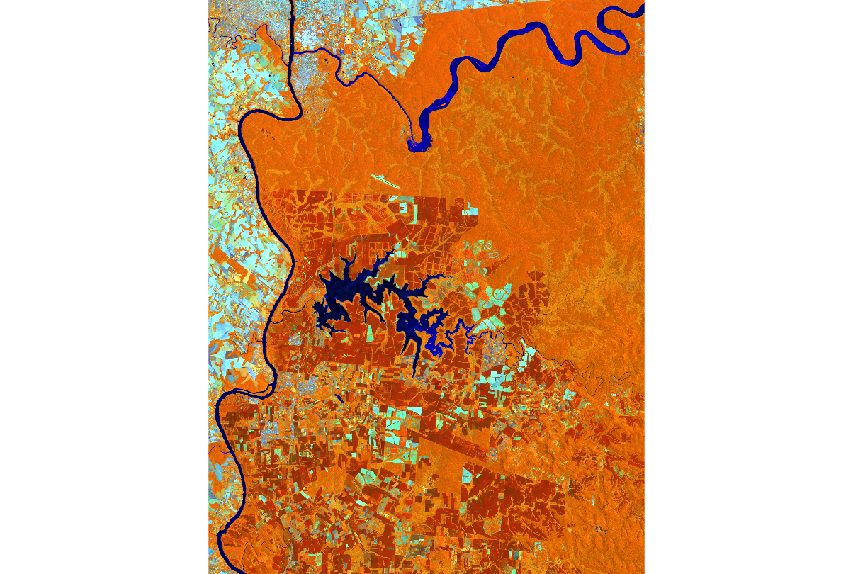
\includegraphics[scale=0.3]{plot453.png}
    \end{center}
    \caption{Combinacion de bandas nir-swir1-red en R.}
    \label{fig:plot453}
    \end{figure}

    Para graficar las bandas por separador hacemos \texttt{plotRGB(ref.2016)}
    (Figura \ref{fig:plotband}).

    \begin{figure}[h!]
    \begin{center}
        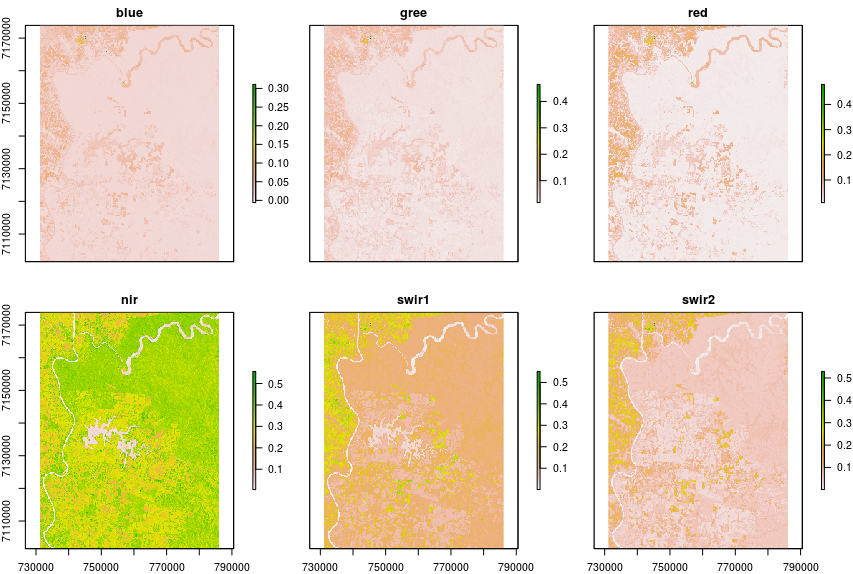
\includegraphics[scale=0.3]{plotband.png}
    \end{center}
    \caption{Gr\'afico de bandas con realce autom\'atico para cada una.}
    \label{fig:plotband}
    \end{figure}

\end{exa}

\begin{act}
   Abra el archivo guardado en QGIS y vuelva a mirar la firma espectral para
   distintas coberturas. ¿Entre que valores se encuentra ahora?
\end{act}

Veamos como trabajar m\'as en detalle con los valores de nuestra imagen.

\begin{exa}

    Hagamos un an\'alisis estad\'istico de la imagen ejecutando el
    comando \texttt{summary(ref.2016)}
    \begin{Verbatim}[fontsize=\small]
               blue   gree    red     nir   swir1   swir2
    Min.    -0.0278 0.0000 0.0000 -0.0128 -0.0069 -0.0038
    1st Qu.  0.0128 0.0328 0.0184  0.2763  0.1198  0.0493
    Median   0.0138 0.0362 0.0203  0.3287  0.1365  0.0572
    3rd Qu.  0.0170 0.0450 0.0329  0.3557  0.1644  0.0749
    Max.     0.5548 0.8257 0.8034  0.7542  0.9181  0.9446
    NA's     0.0000 0.0000 0.0000  0.0000  0.0000  0.0000
    \end{Verbatim}
    Calculamos los histogramas de todas las bandas con el
    comando \texttt{hist(ref.2016)} y el scatter plot entre dos bandas como
  \verb|plot(ref.2016$red,ref.2016$nir)|.

    En caso de querer todos los scatterplots e histogramas en un solo gr\'afico
    usamos el comando \texttt{pairs(ref.2016)}.
    \end{exa}


\section{Manejo vectorial en R}

Hasta ahora estamos analizando la imagen completa, pero podemos analizar
determinadas zonas utilizando un archivo vectorial.. Tambi\'en ser\'a
posible muestrear la imagen usando otro raster, pero lo veremos m\'as adelante.

Para trabajar con vectores en R utilizaremos la libreria
\texttt{library(rgal)}.

\begin{exa}
    Veamos como realizar el an\'alisis b\'asico de un vector en R. Comenzamos
    ley\'endolo

    \begin{lstlisting}
    firmas <- readOGR(dsn="vector\_data/", layer="firmas")
    \end{lstlisting}

    Notamos en este caso que debemos indicar por separado la carpeta que
    contiene al shapefile en \emph{dsn} y el nombre de la capa que queremos
    abrir como \emph{layer}.

    Podemos mostrar las propiedades del vector llamando a la variable
    \texttt{firmas} obteniendo
    \begin{Verbatim}[fontsize=\small]
    class       : SpatialPolygonsDataFrame
    features    : 8
    extent      : 738692.8, 767774.6, 7133396, 7165265  (xmin, xmax, ymin, ymax)
    coord. ref. : +proj=utm +zone=21 +south +datum=WGS84 +units=m +no_defs
                  +ellps=WGS84 +towgs84=0,0,0
    variables   : 3
    names       : id, MC_ID,       Comment
    min values  :  0,     1,          Alto
    max values  :  9,     8, Suelo desnudo
    \end{Verbatim}

    Para graficar los vectores y la imagen juntos hacemos

    \begin{lstlisting}
    plotRGB(ref.2016, stretch="lin")
    plot(firmas,add=TRUE,col='red')
    \end{lstlisting}
    donde la primera l\'inea grafica la imagen de fondo y la segunda agrega el
    shapefile sobre ella.
\end{exa}

\begin{act}
    Muestre las propiedades de la capa raster y vectorial y verifique
    que se encuentren en el mismo sistema de coordenadas.
\end{act}

Veamos como extraer datos de un archivo raster con un vector con la funci\'on
\texttt{extract}. Esta toma dos argumentos, el vector que queremos
utilizar y la capa raster sobre la cual hacer la consulta.

\begin{exa}
    Graficar en un scatterplot de dos bandas mostrando la zona del espacio
    ocupada por una cobertura.
    \begin{lstlisting}
    datos <- extract(ref.2016,firmas)
    \end{lstlisting}
    de esta forma realizamos la extracci\'on de todos los datos de la imagen a una
    lista
    \begin{lstlisting}
    plot(ref.2016$red, ref.2016$nir)
    points(as.data.frame(datos[1])$red, as.data.frame(datos[1])$nir,col="green",
           pch = ".")
    \end{lstlisting}
    Ágregamos el scatterplot al muestreo obteniendo
    \begin{figure}[h!]
    \begin{center}
        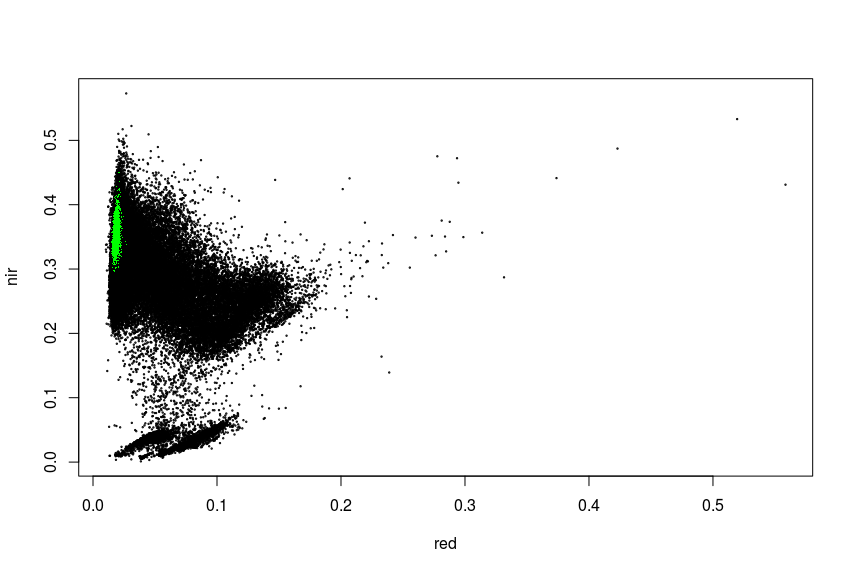
\includegraphics[scale=0.3]{plot-red-nir-zone.png}
    \end{center}
    \caption{Resultado del scatterplot para las bandas roja y nir. Se muestra en
        verde datos correspondientes a la selva paranaense.}
    \label{fig:rednirzone}
    \end{figure}

\end{exa}

La funci\'on \texttt{extract} nos permite tambi\'en aplicar una funci\'on a los datos
extraidos antes de entregarlos al usuario. Veamos como usarla para calcular
datos de interes sobre las coberturas y guardarlo en un archivo vectorial.

\begin{exa}
     Extraer los promedios y desv\'io standar de un raster y agregarlos a un
     vector. Primero extraemos los valores de promedio y desv\'io
     \begin{lstlisting}
     promedio <- extract(ref.2016,firmas,fun=mean)
     desvio <- extract(ref,firmas,fun=sd)
     \end{lstlisting}
     renombramos luego las columnas como promedio y desv\'io seguido de la banda a
     la que pertenecen,
     \begin{lstlisting}
     colnames(promedio) <- paster("mean",colnames("promedio"),sep="_")
     colnames(desvio) <- paster("sd",colnames("desvio"),sep="_")
     \end{lstlisting}
     finalmente agregamos los archivos a un nuevo shapefile
     \begin{lstlisting}
     firmas@data <- cbind(firmas@data,promedio,desvio)
     writeOGR(firmas, sdn="vector_data/processed/,"firmas_datos",
              driver="ESRI Shapefile")
     \end{lstlisting}
\end{exa}

Finalmente, veamos como usar una capa vectorial para graficar las
firmas espectrales y graficarlas para distintas coberturas

\begin{exa}
     Graficar las firmas espectrales en funci\'on de la longitud de onda para cada
     pol\'igono. Utilizaremos dos nuevas librerias,
     \texttt{reshape2} y \texttt{lattice}

     Comenzamos convirtiendo en dataframe a nuestros promedios, donde cada
     columna corresponde a una firma espectral
     \begin{lstlisting}
     df <- t(promedio)
     colnames(df) <- vector@data$Comment
     \end{lstlisting}
     Agregamos luego una columna con las longitudes de onda en nanometros. Luego
     reformamos el dataframe para que podamos subsetearlo, poniendo finalmente
     los nombres a cada columna
     \begin{lstlisting}
     df$wl <- as.matrix(c(485,560,660,830,1650,2215))
     df <- melt(df,id.vars="wl", variable.name="cobertura")
     names(df) <- c("wl","Cobertura","Reflectancia")
     \end{lstlisting}
     El dataframe resultante deber\'ia ser:
     \begin{Verbatim}[fontsize=\small]
          wl     Cobertura Reflectancia
     1   485          Alto  0.012926561
     2   560          Alto  0.034730646
     3   660          Alto  0.018491884
     4   830          Alto  0.354564681
     5  1650          Alto  0.133750642
     ...
     \end{Verbatim}
     Repetimos el proceso para el desv\'io standar
     \begin{lstlisting}
     dfd <- t(desvio)
     colnames(dfd) <- vector@data$Comment
     dfd$wl <- as.matrix(c(485,560,660,830,1650,2215))
     dfd <- melt("wl","Cobertura","Desvio")
     df$desvio <- dfd$desvio
     df$MC_ID <- as.character(vector@data$MC_ID[match(df$Cobertura,
                              vector@data$Comment)])
     \end{lstlisting}
     El resultado ser\'a ahora
     \begin{Verbatim}[fontsize=\small]
          wl     Cobertura Reflectancia       Desvio
     1   485          Alto  0.012926561 0.0007772473
     2   560          Alto  0.034730646 0.0018113004
     3   660          Alto  0.018491884 0.0011561294
     4   830          Alto  0.354564681 0.0166801398
     5  1650          Alto  0.133750642 0.0075157929
     ...
     \end{Verbatim}
     En primer lugar pondremos todas las firmas espectrales juntas, separadas
     por color, con la libreria \texttt{lattice}
     \begin{lstlisting}
     xyplot(Reflectancia~wl, data=df, groups = Cobertura,
            auto.key=list(space="top", columns=4),
            ty=c("l", "p"))
     \end{lstlisting}
     Aqu\'i la primer l\'inea dice que grafiquemos la reflectancia como funci\'on de
     la longitud de onda, obteniendo los datos del dataframe DF y agrupandolos
     seg\'un la columna cobertura. La siguiente l\'inea agrega la leyenda en la
     parte superior de la figura con 4 columnas. Por \'ultimo en la tercer l\'inea
     pedimos que el gr\'afico tenga l\'ineas y puntos (Figura \ref{fig:spectra-1}).

     \begin{figure}[h!]
     \begin{center}
         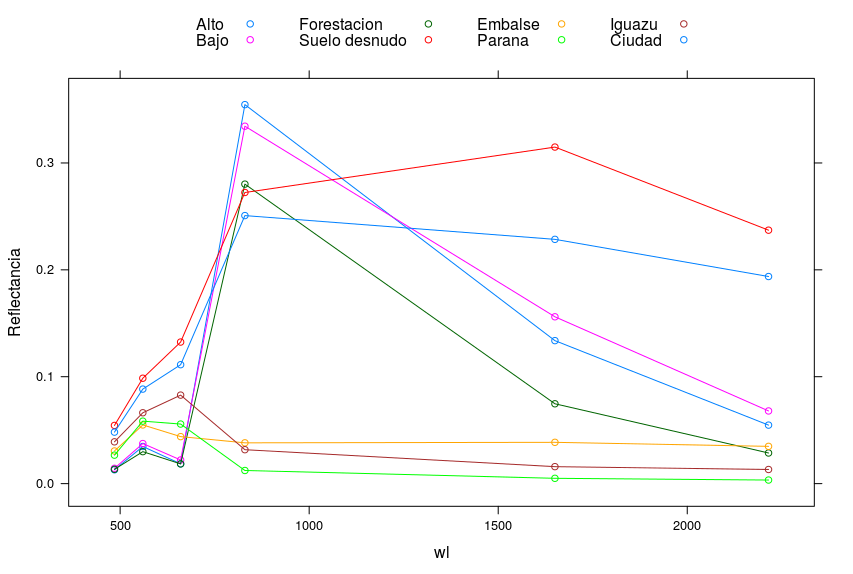
\includegraphics[scale=0.3]{spectra-1.png}
     \end{center}
     \caption{Firmas espectrales}
     \label{fig:spectra-1}
     \end{figure}

     Si queremos agruparlo por categor\'ia de uso y cobertura cambiamos la formula
     \texttt{Reflectancia ~ wl} por \texttt{Reflectancia \~ wl | MC\_ID}
     \begin{lstlisting}
     xyplot(Reflectancia ~ wl | MC_ID, data=df, groups = Cobertura,
            auto.key=list(space="top", columns=4),
            ty=c("l", "p"))
     \end{lstlisting}

     Si queremos graficar solo un subset de datos (Figura \ref{fig:spectra-2}).

     \begin{lstlisting}
     xyplot(Reflectancia~wl | MC_ID, data=df, groups = Cobertura,
            auto.key=list(space="top", columns=4), ty=c("l", "p"),
            subset = Cobertura %in% c("Alto","Bajo"))
     \end{lstlisting}
     \begin{figure}[h!]
     \begin{center}
         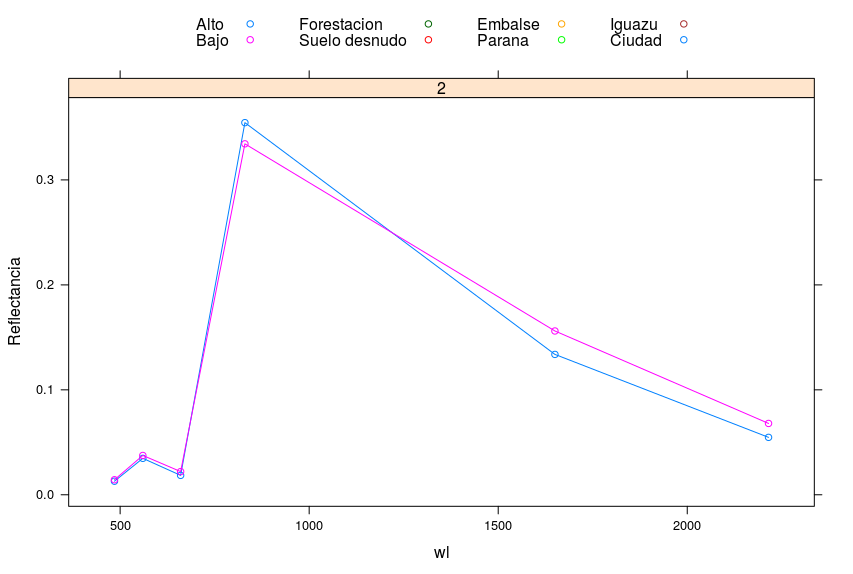
\includegraphics[scale=0.3]{spectra-2.png}
     \end{center}
     \caption{Firmas espectrales}
     \label{fig:spectra-2}
     \end{figure}
 \end{exa}

\begin{act}
    Grafique la media y el desv\'io standar para las distintas coberturas que pudo
     identificar en el punto uno.
\end{act}
